\section{ตัวชี้วัดทางชีวภาพ (Biomarkers)}
ตัวชี้วัดทางชีวภาพ (biomarkers) เป็นตัวบ่งชี้ต่อสภาวะต่างๆ ที่เกิดกับร่างกาย ซึ่งรวมถึงแต่ไม่จำกัดเพียงแต่สถานะการตื่น สภาพอารมณ์
หรือสัญญาณบ่งชี้ของโรค

\section{คลื่นสัญญาณชีวภาพ (Biosignals)}
คลื่นสัญญาณชีวภาพ (biosignals) เป็นคลื่นสัญญาณจากกระแสไฟฟ้าในร่างกาย ซึ่งสามารถตรวจวัดได้ด้วยวิธีการที่ต่างกันไป
และผลจากการตรวจวัดคลื่นแต่ละส่วนจะบ่งบอกซึ่งข้อมูลที่แตกต่างกันออกไปเช่นกัน

งานวิจัยของห้องปฏิบัติการเบรน มุ่งศึกษาคลื่นสัญญาณชีวภาพ Electroencephalography และ

\section{คลื่นไฟฟ้าสมอง (Electroencephalography)}
Electroencephalography หรือ EEG เป็นคลื่นที่เกิดจากการตรวจวัดกระแสไฟฟ้าของสมอง การตรวจวัดโดยมากไม่จำเป็นต้องทำการเจาะผิวหนัง
(noninvasive) โดยใช้อิเล็กโทรดนำไฟฟ้าอ่านคลื่นสมองจากกระโหลก

การตรวจวัดและใช้ข้อมูลจากคลื่น EEG ส่วนมากมุ่งเน้นการใช้ศักย์ไฟฟ้าที่ขึ้นกับเหตุการณ์กระตุ้นของผู้ถูกวัด
(Event Related Potential) กล่าวคือมุ่งสังเกตจุดสูงสุดและต่ำสุดของศักย์ไฟฟ้าของคลื่นสมอง
และหาความสัมพันธ์ระหว่างเหตุการณ์กระตุ้นและการเพิ่มขึ้นหรือลดลงของศักย์ไฟฟ้า

\begin{figure}[h]
	\centering
	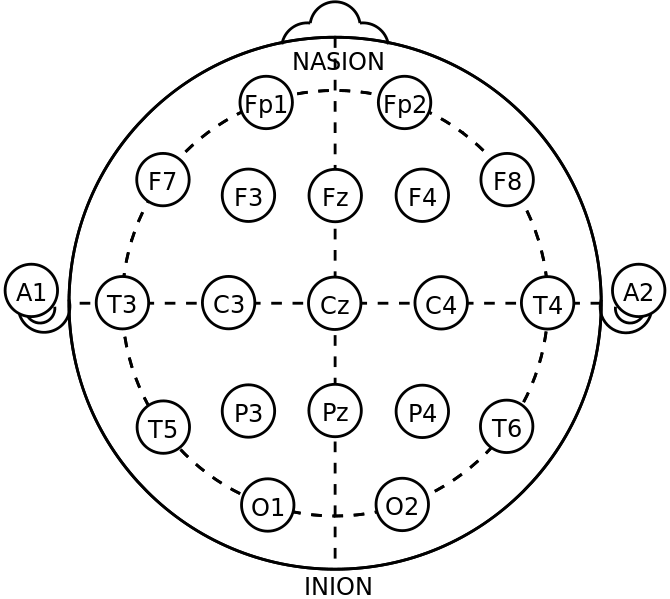
\includegraphics[width=0.5\textwidth]{images/1020.png}
	\caption{ภาพตำแหน่งของการติดขั้วนำไฟฟ้า (electrode) ตามระบบ International 10/20}
	\hspace{\linewidth}
	\textit{รูปภาพประกอบโดยผู้ใช้ Tomaton124 \href{https://commons.wikimedia.org/wiki/File:21_electrodes_of_International_10-20_system_for_EEG.svg}{บนโครงการวิกิมีเดีย คอมมอนส์}
		ชิ้นงานเป็นสาธารณะสมบัติ}
\end{figure}

อย่างไรก็ตาม การใช้คลื่นไฟฟ้านั้นยังสามารถใช้ประโยชน์จากคลื่นส่วนอื่น อันได้แก่คลื่นส่วน Motor Cortex ซึ่งถูกกระตุ้นด้วยการ "จินตนาการ"
การขยับร่างกาย และการใช้คลื่นส่วน Vision Cortex เพื่อกระตุ้นการมองเห็น เช่นการใช้สัญญาณ SSVEP จากสมองส่วนท้ายทอยซึ่งจะสั่นพ้อง
กับการกระพริบของแสงในความถี่ที่ตามองเห็น

\section{คลื่นไฟฟ้าจากการขยับลูกตา (Electrooculography)}
Electrooculography หรือ EOG เป็นคลื่นไฟฟ้าที่เกิดจากการขยับลูกตา โดยหากมองลูกตาเป็นวัตถุที่สามารถหมุนได้ด้วยองศาอิสระ (Degree of Freedom: DOF)
ทั้งหมด 2 องศาอิสระ สามารถจำความรู้นี้มาพิจารณาการใช้คลื่นจากกล้ามเนื้อการกอลกตาในการหาตำแหน่งการกลอกตาได้

\begin{figure}[h]
	\centering
	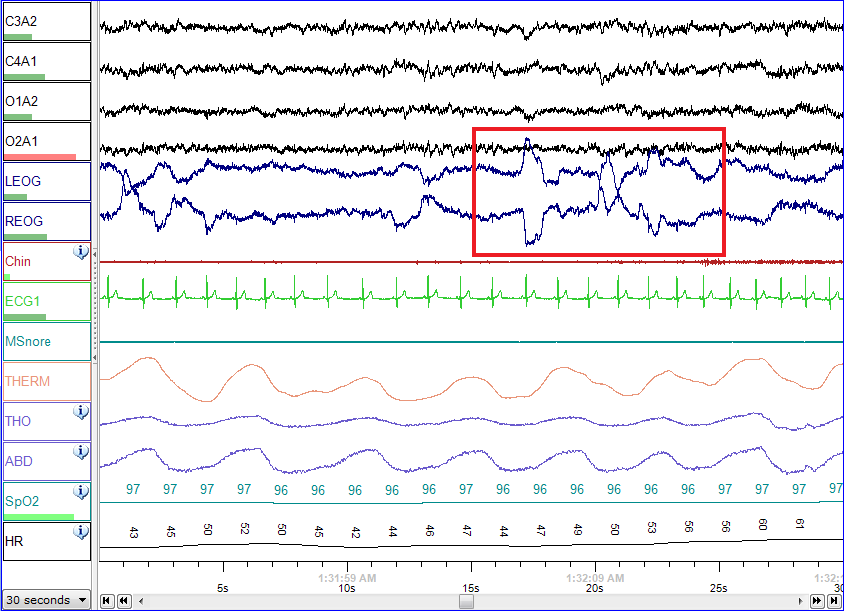
\includegraphics[width=0.7\textwidth]{images/rem_eog.png}
	\caption{ภาพคลื่น EOG ขณะอยู่ในสถานะการนอนหลับ}
	\hspace{\linewidth}
	\textit{รูปภาพประกอบโดยผู้ใช้ NascarEd \href{https://commons.wikimedia.org/wiki/file:sleep\_stage\_rem.png}{บนโครงการวิกิมีเดีย คอมมอนส์}
		สัญญาอนุญาต Creative Commons Attribution-Share Alike 3.0 Unported}
\end{figure}

การวัดคลื่น EOG สามารถทำได้ด้วยการติดอิเล็กโทรดจำนวน 2 คู่ เพื่อวัดการกลอกตาในแนวระนาบ (yaw) และการกลอกตาในแนวดิ่ง (pitch)
โดยค่าที่อ่านได้จากอิเล็กโทรดหนึ่งคู่จะเป็นการกลอกตาในทิศทางหนึ่ง กล่าวคือการวัด EOG มุ่งสนใจความต่างศักย์ไฟฟ้าของอิเล็กโทรดคู่นั้น
โดยการกลอกตาไปทางซ้าย (หรือกาารกลอกตาขึ้น) จะให้ทิศทางของตวามต่างศักย์ไฟฟ้าที่ต่างจากการกลอกตาไปทางขวา (หรือการกลอกตาลง)